\section{Evaluation}
\label{s:ward-eval}

To demonstrate the benefits of \sys's design, this section
answers the following questions:

\begin{itemize}

\item Do \sys's techniques reduce the overhead of mitigations for
system calls?  (\autoref{ss:faster})

\item How do mitigations affect the cost of a world switch?
  (\autoref{ss:world})

\item What are the memory overhead associated with \sys's design?
  (\autoref{ss:memoverhead})

%\item Does \sys's use of the unmapped speculation contract address
%  known transient execution vulnerabilities?  (\autoref{ss:secure})

%% \item Could \sys's design reduce overhead for Linux's systems calls?
%%   (\autoref{ss:linux})
 
\end{itemize}

\begin{figure*}[ht]
  \begin{center}
    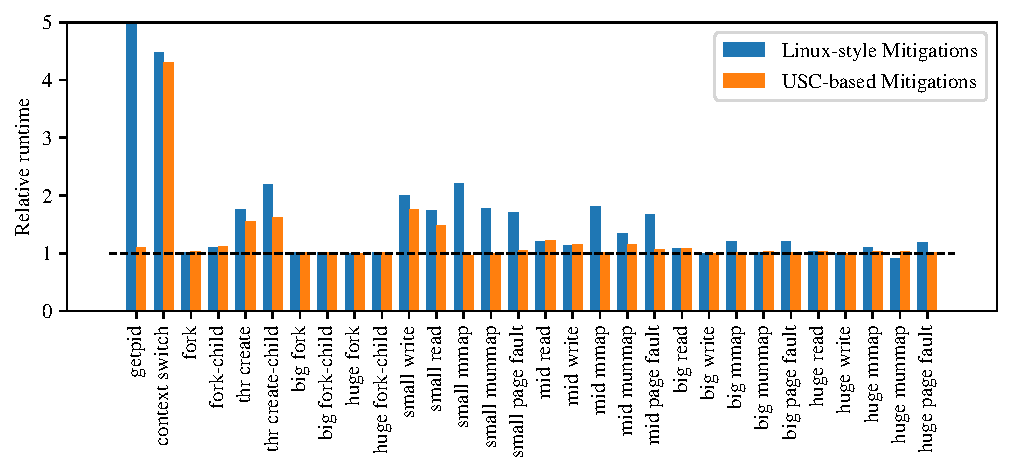
\includegraphics[width=\textwidth]{results/ward_overhead_lebench}
  \end{center}
\vspace{-\baselineskip}
\caption{Performance of \sys with fast USC-based mitigations and with Linux-style mitigations,
  normalized against the baseline performance of \sys without any mitigations.}
\label{fig:slowdown}
\end{figure*}


\subsection{Experimental methodology}

To answer these questions, we consider three different configurations of \sys:

\begin{itemize}
\item Baseline: \sys with no mitigations against side channels.

\item Linux-style: \sys with standard mitigations against side channels,
mirroring the approach taken by the Linux kernel.  This configuration does
not use separate Q domains; all system calls directly enter the K domain.

\item USC-based: \sys with fast mitigations that take advantage of the split
between the Q domain and the K domain, leveraging the \contract{}.  The
K domain implements the same mitigations as in Linux-style.

\end{itemize}

\sys's design is aimed at reducing the overhead of mitigations
associated with system calls.  To zoom in on the system call overhead,
we evaluate \sys's performance using \bench~\cite{lebench}, a
collection of system call workloads representative of a range of real
applications.  This allows us to precisely report and explain the
effect of \sys's techniques on individual system calls.  We don't
report results for the networking benchmarks in \bench, because the
\sys prototype doesn't have a suitable in-kernel network stack.

All benchmarks were run on a Dell PowerEdge T430 with two E5-2640 v4
CPUs and 64 GB of RAM.

%% All benchmarks were run on a 4th Gen Lenovo X1 Carbon Laptop with a Intel
%% i7-6600U CPU and 16 GB of RAM. Except where otherwise noted, we ran with the
%% latest available microcode for our processor (released on Nov 15, 2019).
%% \nz{XXX update to describe bhw2 hardware.}

One potential concern with the use of recent microcode is that it makes
the baseline slower, which in turn makes the cost of mitigations appear
lower than they really are.  This is similar to the significant effect
we observed with newer CPUs, as described in \autoref{s:motivation}.
However, with newer microcode, we find that the performance of the
baseline is not significantly affected: it achieves similar performance
even when we use old microcode.  The reason for this is that the recent
microcode updates add mitigations that can be specifically enabled (e.g.,
through the \texttt{SPEC\_CTRL} MSR), but almost nothing is enabled by
default.  The Linux and Ward baseline experiments do not enable these
mitigations, and thus the performance effect is minimal.
%\nz{perhaps verify this also on bhw2, since we did this experiment
%originally on jonathan's laptop}

For the Linux measurements of \bench, we use the 5.4.0 kernel on Ubuntu 20.04.


\subsection{\sys's USC-based fast mitigations}
\label{ss:faster}

\paragraph{\bench.}

\autoref{fig:slowdown} shows the benefit of \sys's fast mitigations on
\bench.  The figure compares \sys with USC-based and Linux-style mitigations,
relative to the baseline with no mitigations.
As shown, \sys with fast USC-based mitigations is often able to
match the unmitigated baseline.  The reason is that many of the microbenchmarks can
execute with no or very few world switches, as shown in
\autoref{fig:count}.

Many microbenchmarks (\texttt{getpid} through \texttt{huge pagefault}
in \autoref{fig:count}) have nearly 0 transparent and intentional
world switches. They execute completely in the Q domain. The
reason that some have near 0 world switches, but not exactly 0, is
that during the measurement they were interrupted by a timer
interrupt, which requires a world switch to the K domain to run the
scheduler (the remainder of the syscall is then executed in the K
domain too).

Another cause for fractional numbers of transparent world
barriers is that some operations might have a slow path that requires
secrets but only gets triggered infrequently (i.e. because a memory
allocator pool ran empty). A strength of the \sys approach is that these
sorts of cases don't have to be manually annotated and in fact it is
harmless to completely ignore them provided they are executed infrequently
enough.

There are several microbenchmarks (e.g., the bigger \texttt{read} and
\texttt{write} ones) that perform one intentional world switch per
system call.  These system calls immediately enter the K domain and
thus perform identical to \sys with full mitigations, and have the
same overhead.  These system calls also perform much work in the kernel and
the overhead of the 1 world switch is amortized by that work.

\begin{figure}
\small
\centering
\begin{tabular}{lrccc}
  & {\bf \# sys calls} & \multicolumn{3}{c}{{\bf World switches}} \\
  & & {\bf T} & {\bf I} & {\bf Sum}  \\
  \midrule
getpid & 1 & 0 & 0 & 0 \\
small write & 1 & 0 & 0 & 0 \\
small read & 1 & 0 & 0 & 0 \\
small mmap & 1 & 0 & 0 & 0 \\
small munmap & 1 & 0 & 0 & 0 \\
small page fault & 1 & 0 & 0 & 0 \\
mid mmap & 1 & 0 & 0 & 0 \\
mid munmap & 1 & 0 & 0 & 0 \\
mid page fault & 1 & 0 & 0 & 0 \\
big mmap & 1 & 0 & 0 & 0 \\
big page fault & 1 & 0 & 0 & 0 \\
huge mmap & 1 & 0 & 0 & 0 \\
huge page fault & 1 & 0 & 0 & 0 \\
context switch & 2 & 0 & 1 & 1 \\
thr create & 3 & 0 & 1 & 1 \\
thr create-child & 4 & 0 & 1 & 1 \\
mid read & 1 & 0 & 1 & 1 \\
mid write & 1 & 0 & 1 & 1 \\
big read & 1 & 0 & 1 & 1 \\
big write & 1 & 0 & 1 & 1 \\
big munmap & 1 & 1 & 0 & 1 \\
huge read & 1 & 0 & 1 & 1 \\
huge write & 1 & 0 & 1 & 1 \\
huge munmap & 1 & 1.001 & 0 & 1.001 \\
fork & 2 & 0 & 2 & 2 \\
big fork & 2 & 0 & 2 & 2 \\
huge fork & 2 & 0 & 2 & 2 \\
huge fork-child & 17 & 0 & 7 & 7 \\
big fork-child & 17 & 0.006 & 7.02 & 7.026 \\
fork-child & 17 & 0.012 & 7.065 & 7.077 \\
\end{tabular}
\caption{The microbenchmarks, sorted by the sum of the number of transparent
  ({\bf T}) and intentional ({\bf I}) world switches per iteration, along
  with the number of system calls invoked (including page faults).}
\label{fig:count}
\end{figure}

The \texttt{thr create} and \texttt{thr create-child} do multiple syscalls
per iteration, but average  one world barrier per iteration.
Specifically, the \texttt{thr create} microbenchmark makes three systems calls:
one \texttt{clone} that requires a world switch and a call to each of
\texttt{sigprocmask} and \texttt{set\_robust\_list} which don't. The
\texttt{thr create-child} microbenchmark includes an additional call to
(\texttt{sigprocmask}) from the child process, for which \sys can also
avoid the world switch.

The \texttt{fork} and \texttt{fork-child} benchmarks each do a single syscall
with an intentional world barrier that takes the vast majority of execution time,
but also raise a handful of page faults to populate page table entries (which
need secrets if they are copy-on-write related or if the kernel runs out of
zeroed memory pages and has to prepare more).

An interesting case is the \texttt{context switch} microbenchmark.
This microbenchmark measures context switching by writing and reading
a byte over a pipe between two processed pinned to the \textit{same}
core. The \texttt{write} calls avoids a world switch because the
scheduler can wake other processes while in the Q domain, but the
\texttt{read} call causes a context switch and (since the two
processes are mutually distrusting) thus requires a world switch.

When we modify the microbenchmark to pin the two processes to \textit{different}
cores we observe that it runs without world switches and that the overhead is about 25 times lower than Linux-style mitigations.

%% When measuring context switching overhead for ping-ponging a futex between two
%% threads of a user-level process, fast mitigations improve performance: fast
%% relative to no mitigations has a performance slow down of 1.14$\times$, while
%% standard mitigations have a slow down of 2.79$\times$. \jb{Replace with pipes
%%   benchmark}

%% schedbench.csv


\paragraph{Application: git.}

To confirm that the improved performance of \sys's fast mitigations seen
in \bench translates into application-level performance improvements,
we evaluated the performance of \texttt{git}.  For this benchmark, we
ran \texttt{git status} in a 100 MB repository that we cloned from
GitHub; all of the file system
state was cached in memory. The average runtime for Linux-style mitigations
took 24.6\%
longer than the unmitigated baseline, and USC-style mitigations took 11.2\% longer than
the unmitigated baseline.
Much of the speedup is due to the fact that \texttt{git status} invokes
frequent \texttt{lstat} system calls, which can execute in the Q domain.
The remaining overhead is due to system calls like \texttt{openat} that
require a world barrier for accessing potentially sensitive file contents.


\subsection{World switch}
\label{ss:world}

\begin{figure}
\small
\centering
\begin{tabular}{lrr}
  {\bf Configuration}
  & {\bf Transparent} & {\bf Intentional} \\
\midrule
None & 2457 cycles & 1082 cycles \\
SpectreV2 & 2453 cycles & 1075 cycles \\
MDS & 3337 cycles & 1980 cycles \\
MDS+SpectreV2 & 3363 cycles & 1992 cycles \\
MDS+SpectreV2+Q\_\texttt{retpoline} & 3406 cycles & 2014 cycles \\
\end{tabular}
\caption{The costs of transparent and intentional world switches for
  different configurations.}
\label{fig:barrier}
\end{figure}

\autoref{ss:faster} shows that the mitigation overhead is dominated by
the cost of a world switch.  This section breaks down this cost.

An intentional world switch via \texttt{kswitch()} takes around 644
cycles on a shallow stack, plus 50 cycles or so for every KB of stack
used (the cost of a \texttt{memcpy}). A transparent world switch using a page
fault adds 1372 cycles.

\autoref{fig:barrier} measures the cost of a null system call that
invokes an intentional or a transparent world switch, and returns.  It
shows the cost for different configurations: no mitigations, MDS
mitigations, SpectreV2 mitigations, and with \texttt{retpoline} in Q
domain.  The configuration with Q\_retpolines runs with retpolines
in both the Q and K domains. It shows the benefit of \sys patching
them out at runtime: the retpoline that disables branch prediction
for indirect jumps through the system call table costs 22 cycles.


\subsection{\sys memory overhead}
\label{ss:memoverhead}

Because the memory protection mechanisms that \sys uses to expose non-secret
data to Q domains operates on a 4KB or 2MB granularity, \sys's approach incurs
some additional memory overhead. Figure~\ref{fig:memoverhead} lists some of
these cases. In general we face a trade-off when filling small dynamic memory
allocations for Q domain state: either we use an entire page each time, or we
tolerate higher memory fragmentation because all chucks of memory on a page must
be only used by the same Q domain.

\begin{figure}[t]
\small
\centering
\begin{tabular}{@{}lll@{}}
  {\bf Component} & {\bf Overhead} & {\bf Explanation} \\
  \midrule
  Kernel text & 2 MB & Separate text segments for \\ && \quad Q and K domains \\
  Public kernel data & < 4 KB & Padding to a page boundary \\
  Process structure & 4 KB / process & Allocated on its own page \\
  Thread structure & \textasciitilde 6 KB / thread & Split between a Q domain \\ && \quad page and a K domain page \\
  Q domain stack & 32 KB / thread & Smaller stacks possible by \\ && \quad avoiding deep recursion \\
  Page tables & \textit{varies} & Q domain mappings require \\ && \quad additional PTEs \\
  Inodes & -- & Many public allocations \\
  Scheduler state & -- & \quad packed into a single page \\
\end{tabular}
\caption{Memory overhead of different \sys components.}
\label{fig:memoverhead}
\end{figure}

\subsection{Security}
\label{ss:secure}

%\paragraph{\sys mitigations work.}

To validate that \sys's mitigations work, we implemented a demonstration
program that attempts to execute a Spectre V2 attack against the \sys kernel.
While running with applicable mitigations disabled (i.e. each Q and K domain
retpoline replaced with a normal indirect jump) the attack succeeds in
exfiltrating secret kernel data. However, when our Spectre V2 mitigations are
re-enabled (by re-enabling retpolines in the K domain) the attack is thwarted.
It is of course impossible to be certain that all variations on the attack
would be blocked, but this test provides some confidence both that the unmitigated
baseline is vulnerable to transient execution attacks, and that \sys is able to prevent
them.


%% \paragraph{\contract covers known attacks.}

%% We next examine the question of whether known transient execution attacks
%% (see \autoref{fig:mitigations}) violate the \contract.
%% As noted before, the original Meltdown attack does
%% not conform because it allows speculative access to pages of memory that should
%% be inaccessible to the current context. For \sys this violation actually turns
%% out to be irrelevant (because preventing secrets from leaking between the K and
%% Q domains does not rely on the User bit in the page table entries). However,
%% Intel's rapid deployment of hardware fixes shows both that it does consider this
%% to be a bug, and that changes to restore the \contract were straightforward
%% compared to some of the other attacks which still haven't been fully resolved in
%% new hardware.

%% L1TF predominantly impacts virtual machines (which \sys doesn't support) but is
%% an interesting case to analyze. From one perspective it violates the contract
%% since it allows a guest VM to read any data at physical address --- even data
%% that should be inaccessible per the second level page table. But another
%% perspective is that it only applies to data already in the L1 cache that should
%% only have been loaded in if there was a valid page table mapping, so the
%% \contract does hold. In this view, the L1 cache is just more microarchitectural
%% state that must be flushed if it is potentially contaminated by secrets.  In
%% either case, Intel has treated L1TF as bug and patched it in new hardware.

%% Existing Spectre style attacks don't violate the \contract because they require
%% secret data to be architecturally visible to the victim code.


%% \begin{figure}
%% \centering
%% \begin{tabular}{lcc}
%% {\bf Vulnerability} & \multicolumn{2}{c}{{\bf Addressed by \contract{}}} \\
%%  & on AMD & on Intel \\
%% \midrule
%% Spectre & Yes & Yes \\
%% Meltdown & Yes & w/ hardware fix \\
%% L1TF & Yes & w/ hardware fix \\
%% RIDL & Yes & Yes \\
%% Fallout & Yes & Yes \\
%% ZombieLoad & Yes & Yes \\
%% ... other attacks: LVI?
%% \end{tabular}
%% \caption{A qualitative evaluation of transient execution vulnerabilities
%%   and whether they are prevented by \sys's use of \contract{} on AMD and
%%   Intel processors.}
%% \label{fig:attackeval}
%% \end{figure}

%% \subsection{Linux}
%% \label{ss:linux}

%% To gauge whether we could expect similar improvements for fast
%% mitigation for Linux, we compare the overheads of full mitigations for
%% \sys and Linux (as reported in \autoref{fig:linuxslowdown} in
%% \autoref{s:motivation}).  If the mitigation overheads in \sys are much
%% higher than Linux's, then we might not expect improvement in Linux; on
%% the other hand, if they are similar, then \sys's numbers are
%% promising.

%% \autoref{fig:ward_linux_slowdown} shows the results.

%% We cannot directly compare the performance of \sys and Linux, because
%% \sys's implementation of the system calls that \bench stresses is not
%% a sophisticated and complete as Linux's.

%% \fk{getpid we do less work and Linux only marginally more, but because
%%   getpid is little work that different becomes large}

%% \fk{what is going on with on thread create?  \sys is much faster.}

%% \fk{what is going on with munmap benchmarks?}



%% \begin{figure*}[t]
%%   \begin{center}
%%     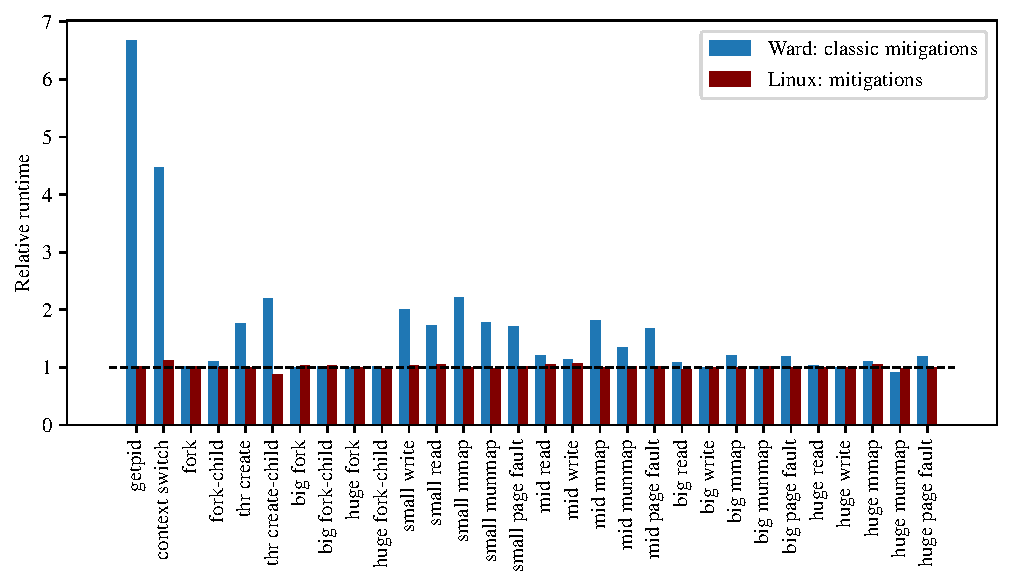
\includegraphics{results/ward_linux_overhead_lebench}
%%   \end{center}
%% \caption{Overheads for full mitigations for \sys and Linux}
%% \label{fig:ward_linux_slowdown}
%% \end{figure*}

%% The baselines for \autoref{fig:ward_linux_slowdown} are \sys and Linux
%% without mitigations. \autoref{fig:ward_linux} shows the relative
%% performance of \sys vs. Linux.

%% \fk{explain radixtree code to address big/huge mmap and fork.  issue:
%%   radix tree can merge 128 pages, but not merged more work (e.g., ref
%%   count) same per 512x128.  benchmarks does 10,000, merge per 128
%%   pages. increase fanout would allow us to do better.}



%% \begin{figure*}[t]
%%   \begin{center}
%%     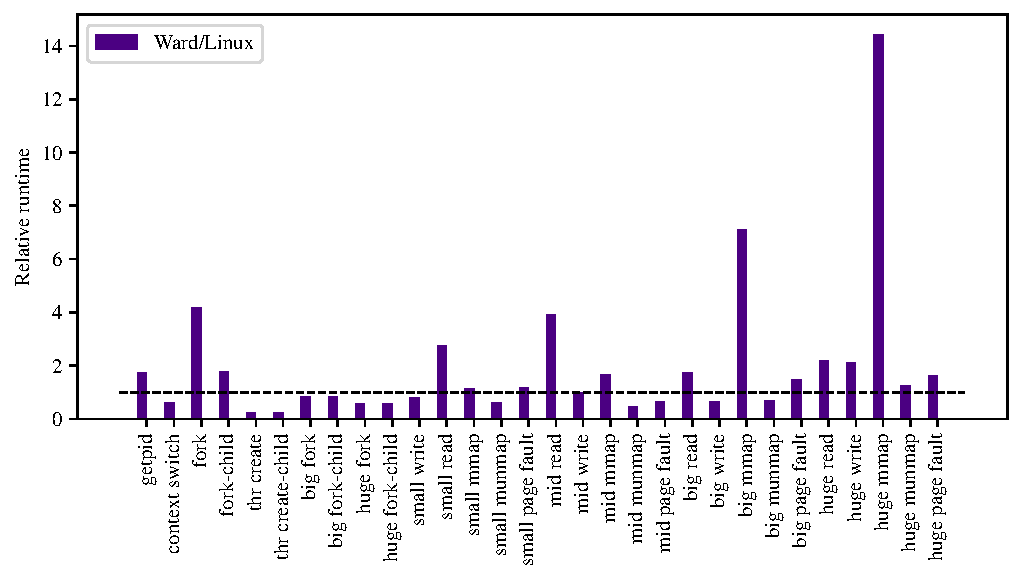
\includegraphics{results/ward_linux_lebench_no_mitigations}
%%   \end{center}
%% \caption{\sys relatative to Linux with no migitations.}
%% \label{fig:ward_linux}
%% \end{figure*}


